% !TEX root = ../thesis.tex
    
%**************************************************************
% Introduzione
%**************************************************************

\chapter{Introduzione: anomaly detection} \label{cap:intro}
    I sistemi complessi sono ubiqui nell'industria moderna e nei servizi dai quali tutti noi traiamo vantaggio 
    quotidianamente. La complessità di 
    tali sistemi i quali, di norma, prevedono la ricezione e l'elaborazione di un certo input, adempiono a task 
    potenzialmente ortogonali e, spesso, processano dati potenzialmente eterogenei ricavati dalla grande 
    quantità di dispositivi e sensori connessi, suscita inquietudini su potenziali anomalie che possono avere
    fonti e natura varie; che sia per il malfunzionamento di uno dei componenti propri del sistema o 
    dei suoi dispositivi connessi, o deviazioni nella natura del dominio del sistema. 
    
    In linea generale, i dati estratti delineano il ciclo di vita del sistema ed è cruciale identificare tempestivamente
    qualsiasi irregolarità per identificare la radice del problema e 
    contestualmente prevenire o minimizzare perdite; perdite la cui rilevanza può essere di natura finanziaria, 
    dove pochi minuti di malfunzionamenti potrebbero tradursi in danni economici di cifre a sei o sette zeri. In sistemi ancora 
    più delicati, come quelli presenti su un aereomobile, tali perdite potrebbero persino mettere a 
    rischio la vita dei passeggeri e dell'equipaggio di volo.

    Di solito, le serie temporali multivariate presentano un certo grado di rumore nelle applicazioni del 
    mondo reale. Pertanto, i modelli concepiti per affrontare il problema della rilevazione di anomalie devono 
    essere sviluppati prendendo in seno tale eventualità. Sarebbe auspicabile che gli algoritmi di 
    detection potessero definire una misura numerica dei punti anomali basata sulla gravità degli eventi 
    che hanno originato tali anomalie. In questo modo, le aziende e gli operatori potrebbero agire in modo 
    relativo e dinamico per risolvere il problema e, potenzialmente, prevenire l'insorgere di un'anomalia 
    prima che essa si manifesti.

    I ricercatori hanno esplorato e implementato modelli incentrati sui dati per l'identificazione e l'analisi 
    di anomalie e negli ultimi anni la questione, grazie a tecniche avanzate di machine learning e deep 
    learning e amplificata dalla moltitudine di dati collezionati, è diventata sempre più saliente. 


    Le anomalie possono essere suddivise in tre macrocategorie:
    \begin{enumerate}
        \item \textbf{Anomalie a punto} che corrispondono a singoli dati nel tempo considerati "outlier"
            poiché si discostano significativamente dal comportamento standard del resto del dataset. 
            La \hyperref[fig:point-anomaly]{Figura 1.1} 
            illustra un esempio di un dataset in cui si è verificata un'anomalia di tipo puntuale. Possiamo
            notare che un'osservazione, quella evidenziata in rosso, ha un valore notevolmente superiore 
            rispetto al resto del dataset.
            \begin{figure*}[htb]
                \centering
                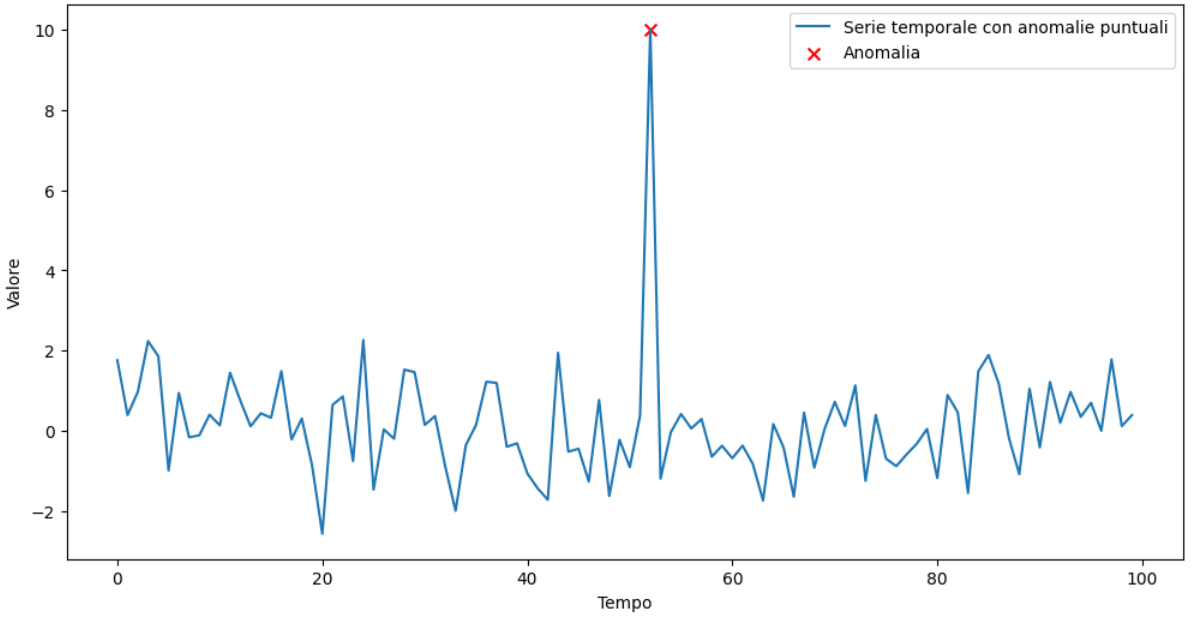
\includegraphics[width=0.6\textwidth]{./input/chapters/figs/point-anomaly.png}
                \caption{Dataset sintetico con anomalia a punto. Il dataset, ad esempio, potrebbe rappresentare il grado 
                di performance di un atleta in un intervallo di cento giorni. L'anomalia puntuale potrebbe indicare un 
                errore nell'inserimento dei dati.}
                \label{fig:point-anomaly}
            \end{figure*}
        \item \textbf{Anomalie contestuali} le quali rappresentano punti, o sequenze di punti, differenti 
        o distanti dal resto del dataset ma solo se presi in considerazione in un contesto specifico, che sia
        spaziale o temporale. 
        La \hyperref[fig:contextual-anomaly]{Figura 1.2.} fornisce un esempio di due anomalie di un dataset 
        sintetico che rappresenta l'indice di temperatura in una finestra temporale lunga due anni. 
        Questi punti, quando considerati nel loro contesto temporale, risultano essere anomalie; 
        tuttavia se analizzassimo complessivamente il dataset senza tener conto dell'ordinamento temporale, 
        essi non sembrerebbero affatto fuori dall'ordinario.

        \begin{figure}[H]
            \centering
            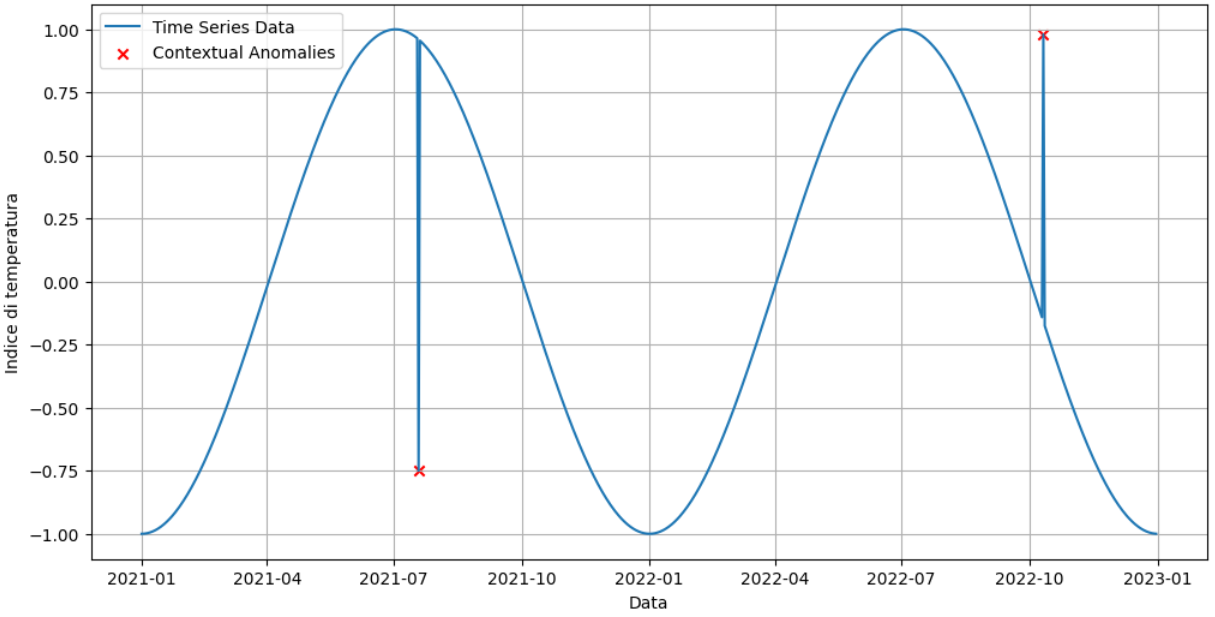
\includegraphics[width=0.6\textwidth]{./input/chapters/figs/contextual-anomaly.png}
            \caption{Dataset sintetico con anomalie contestuali. Il dataset rappresenta un indice di temperatura
            lungo due anni. Le anomalie contestuali nell'esempio registrano un grado di temperatura molto più bassa della norma a luglio e 
            una temperatura molto più alta a ottobre.} 
            \label{fig:contextual-anomaly}
        \end{figure}     
    
        \item \textbf{Anomalie collettive} si riferiscono a modelli che coinvolgono insiemi di osservazioni divergenti 
        rispetto al resto del dataset. Per esempio, la \hyperref[fig:collective-anomaly]{Figura 1.3.} presenta una 
        serie temporale contenente una sottoserie temporale evidenziata in rosso, la quale si differenzia dalle 
        altre sottoserie. In un contesto ipotetico, questa situazione potrebbe rappresentare un contatore bloccato 
        con problemi nell'aggiornamento dei dati.

        \begin{figure}[H]
            \centering
            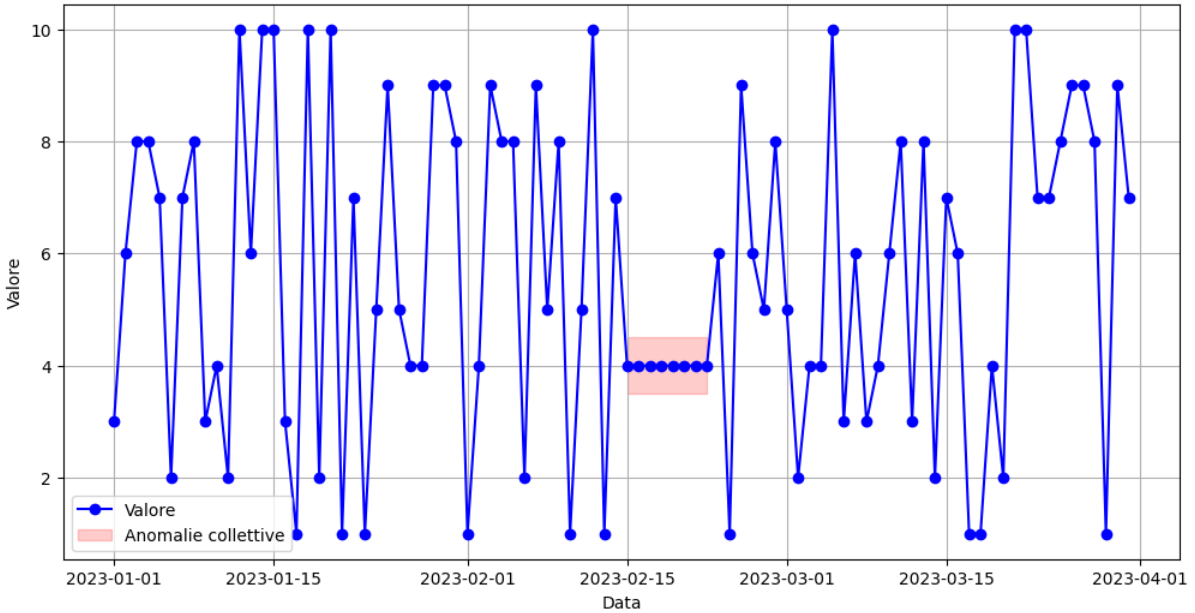
\includegraphics[width=0.6\textwidth]{./input/chapters/figs/collective-anomalies.png}
            \caption{Dataset sintetico con anomalie collettive. Il dataset può essere visto come la rappresentazione di un contatore il quale, 
            nel momento in cui avvengono le anomalie collettive, rimane bloccato.}
            \label{fig:collective-anomaly}
        \end{figure}   
    \end{enumerate}
    L'individuazione delle anomalie nell'ambito del machine learning, come chiaramente 
    illustrato nei precedenti esempi, è influenzata da una serie di fattori.
    Se tali fattori non vengono considerati in fase iniziale, potrebbero condurre a un'analisi poco accurata o addirittura errata. 
    Come si sottolinea in modo particolare nella \hyperref[fig:contextual-anomaly]{Figura 1.2.} e nella 
    \hyperref[fig:collective-anomaly]{Figura 1.3.}, i modelli devono tener conto della dipendenza temporale 
    delle osservazioni. Nella \hyperref[fig:temporal-dependency]{Figura 1.4.} è mostrato un semplice esempio
    di dipendenza temporale: il prezzo delle azioni a tempo $t$ dipende dal prezzo al tempo $t-1$ e influenza 
    il prezzo del tempo $t+1$. I modelli, inoltre, devono essere sviluppati sulla base che i dati su cui saranno addestrati 
    possono vivere in contesti multivariati; è bene che gli algoritmi osservino i vari segnali di un dataset 
    prendendo in considerazione la loro correlazione.

\begin{figure}[H]
    \centering
    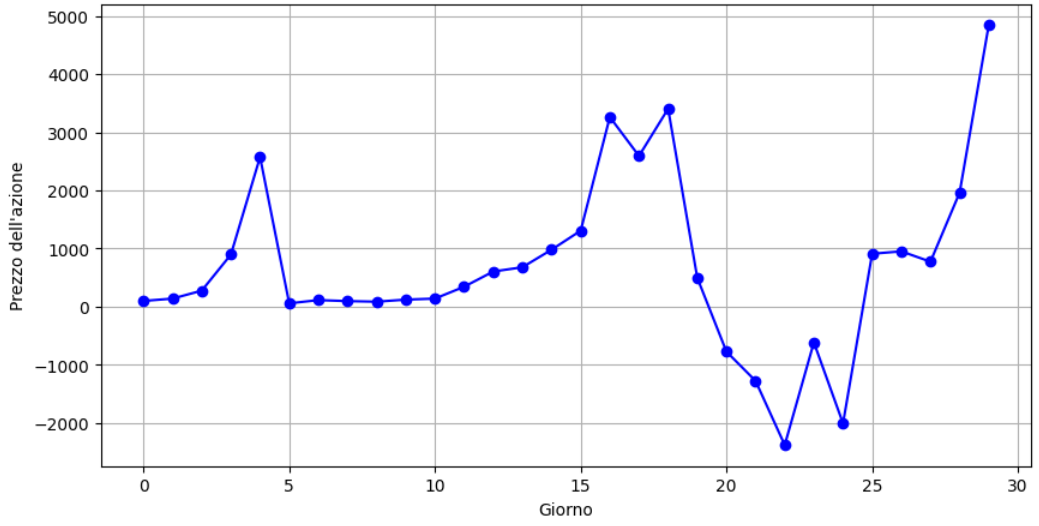
\includegraphics[width=0.6\textwidth]{./input/chapters/figs/temporal-dependency.png}
    \caption{Dataset sintetico con dipendenza temporale rappresentante un prezzo di un'azione nel tempo. La dipendenza temporale è dovuta
    al fatto che il prezzo in un generico tempo $t$ influisce sul prezzo al tempo $t+1$.}
    \label{fig:temporal-dependency}
\end{figure}    

    Il problema della rilevazione delle anomalie può essere affrontato mediante un approccio supervisionato, 
    il cui obiettivo è classificare in modo arbitrario le osservazioni anomale da quelle non anomale. 
    La peculiarità di questo approccio è che le anomalie, per essere definite tali, rappresentano una minoranza 
    all'interno del dataset.

    Un approccio non supervisionato è preferibile per il problema dell'individuazione delle anomalie. Algoritmi 
    diversi che utilizzano metodologie varie, come quella statistica con Auto Regressive Moving Average\cite{arma} (ARMA) e quella del machine learning per algoritmi come 
    One-Class Support Vector Machine\cite{ocsvm} (OC-SVM), o il deep learning con Telemanom\cite{telemanom} e MSCRED\cite{mscred}
    cercano di discriminare le anomalie dalle osservazioni non anomale senza la necessità di disporre
    delle etichette ground-truth, ma basandosi esclusivamente sull'analisi della serie 
    temporale di interesse. Questo metodo, oltre a essere più idoneo, semplifica notevolmente 
    la fase di preparazione dei dati escludendo la costruzione delle etichette.

    La tesi è strutturata in cinque capitoli.
    \begin{enumerate}
        \item Nel primo capitolo, quello corrente, viene fatta una piccola paronamica riguardo al problema dell'analisi delle anomalie.
        \item Nel secondo capitolo vengono osservate le metriche e la finestra temporale del dataset di Infostud su cui si 
                sono svolti gli esperimenti e vengono giustificate le ragioni per cui è stato scelto quel dataset in particolare.
        \item Il terzo capitolo illustra le varie metodologie applicate per la risoluzione del problema dell'anomaly detection
                al prezioso dataset di Infostud, per auspicabilmente risolvere e tracciare anomalie ai fini del miglioramento 
                della piattaforma più cara a tutta la comunità accademica de La Sapienza. Verranno illustrate le applicazioni di 
                tre approcci diversi: statistico, machine learning e deep learning.
        \item Nel capitolo quattro verranno presentate le metriche di valutazione ai fini di giudicare le performance delle soluzioni 
                dei vari algoritmi. Nello stesso capitolo, verranno anche mostrati i risultati dei vari modelli utilizzati.           
        \item Nell'ultimo capitolo sono riportate e confrontate le conclusioni dei modelli analizzati.           
    \end{enumerate}


    Tutti gli esperimenti citati in questa relazione sono disponibili su 
    GitHub\footnote{https://github.com/Pikarz/tirocinio\_infostud} al link riportato a piè di pagina.